\chapter{Tannu-Tuva}

\lettrine{T}{he postage stamps of Tannu Tuva} form one of philately's curious byways, featuring quirky and colorful stamps, many of questionable validity, issued by an obscure country which held special fascination for young stamp collectors in the middle of the twentieth century.

\begin{comment}
Lorem ipsum dolor sit amet, consectetur adipiscing elit. Sed nibh justo, dictum sed cursus ac, lobortis et lacus. Vestibulum vitae justo enim. Quisque laoreet elementum felis, ut sodales arcu viverra a. Sed molestie odio vulputate sem rutrum a sagittis est rutrum. Morbi dapibus hendrerit magna, sit amet commodo massa posuere sit amet. Duis pharetra quam scelerisque est lobortis fringilla. Maecenas venenatis feugiat lectus, vel facilisis odio pharetra quis. Etiam at nisl eros, sit amet suscipit lorem. Lorem ipsum dolor sit amet, consectetur adipiscing elit. Sed augue nunc, ornare eget congue sit amet, laoreet vel augue. Morbi vel justo quis ipsum adipiscing egestas vitae non est. Vivamus ac quam quam. Nullam pharetra
                                                    interdum mauris, rutrum pulvinar ligula condimentum id. Donec et blandit lorem. 
\end{comment}

\begin{figure}[htp]
\centering
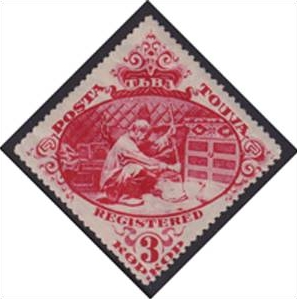
\includegraphics[width=.35\textwidth]{../tannu-tuva/interior-of-tent.jpg}
\caption{RUSSIA TANNU TUVA Diamond shape stamp showing interior of tent.}
\end{figure}


Tannu Tuva was an autonomous region in central Asia between Russia and Mongolia, which in 1921, under Russian instigation, became the Tuvan People's Republic. 



\begin{figure}[htp]
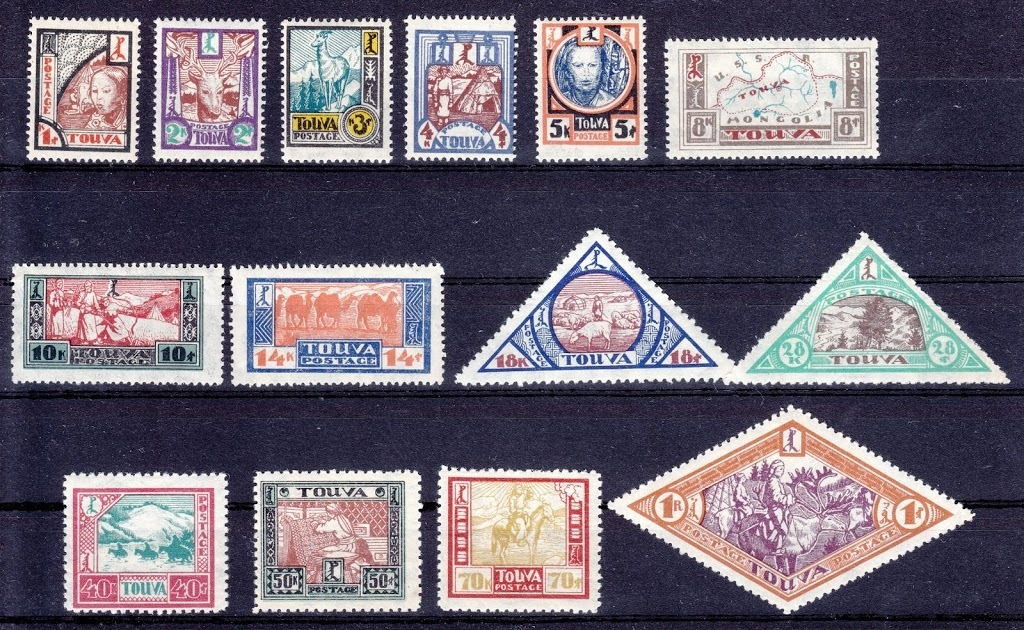
\includegraphics[width=.80\textwidth]{../tannu-tuva/1937-set.jpg}
\caption{RUSSIA TANNU TUVA 1927 Mi 15-28 MLH USD50}
\end{figure}


A treaty between the Soviet Union and the Mongolian People's Republic in 1926 affirmed the country's independence, although no other countries formally recognized it. In 1944, it was annexed to the Soviet Union as part of the Tuvan Autonomous Oblast and in 1961 became the Tuva Autonomous Soviet Socialist Republic. Its successor since 1992, the Tuvan Republic, is a member of the Russian Federation.

\section{Stamps}

Between 1926 and 1933, Tannu Tuva issued 38 postage stamps.[1] The first series depicted the Buddhist wheel of life with Mongolian writing and numerals only. Beginning in 1927, Tannu Tuva issued a series of color stamps with local scenes or a map of the country. These stamps were issued in several shapes, including rectangles, triangles and diamonds, and bore text in Mongolian and the words "TOUVA" and "postage".
From 1934 to 1936, Tuva issued about 100 different postage stamps with exotic images of Tuvan life, including horse racing, nomadic battle scenes, and domestic animals including camels and oxen.[2] 

\begin{marginfigure}
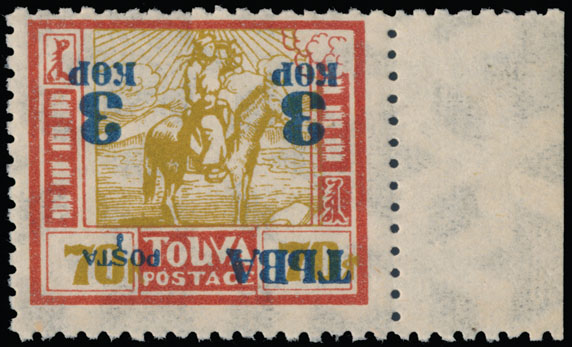
\includegraphics[width=0.95\linewidth]{../tannu-tuva/31a.jpg}
\caption{1442	 31a	
1932, Horseman, inverted blue surcharge 3k on 70k red and olive brown, right sheet margin copy, full OG, NH, VF, C.v. USD 600
130.00 raritan
}
\end{marginfigure}


These large format stamps came in a variety of shapes including diamonds, and were widely sold to collectors in canceled to order form.


These "stamps" were the brainchild of Bela Sekula, a promotor of philatelic "rarities", who in 1934 convinced the Tuvan and Soviet authorities to manufacture exotic stamps to sell to collectors.[2] They were in fact "designed in Moscow, printed in Moscow, franked in Moscow and sold abroad by a Moscow state trading firm to earn hard currency for Moscow."[3][4] Nor were all the images on the stamps accurate representations of Tuvan life. One of the stamps, for example, depicted a "camel racing locomotives along Tuva's nonexistent railway".[5]

\begin{marginfigure}
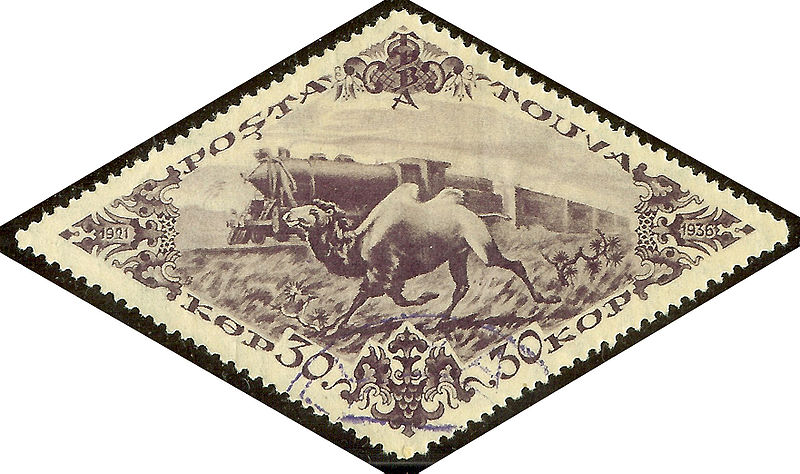
\includegraphics[width=0.95\linewidth]{../tannu-tuva/tuva-camel.jpg}
\caption{
Tuva "stamp" (camel "racing" locomotive) 1936.
}
\end{marginfigure}


The standing of the Tannu Tuva stamps has been controversial. Some catalogues list them as valid postage stamps (Yvert, Michel, Sanabria, and Whitfield King catalogues)[6] while the Scott and Stanley Gibbons catalogues do not recognize these as such.[7][8] 

\begin{figure}[htp]
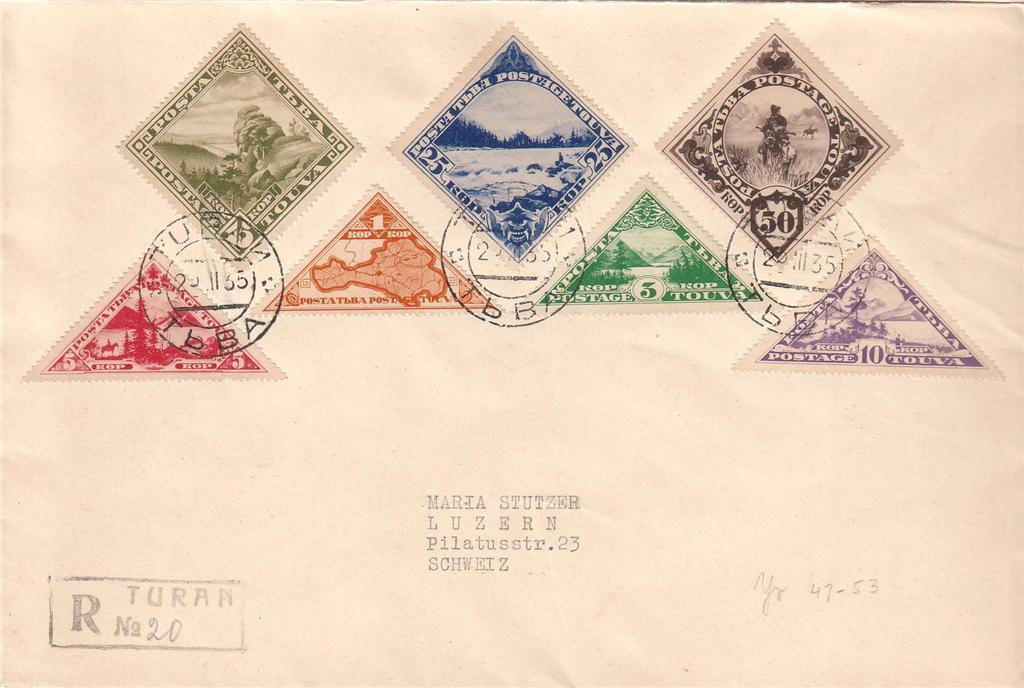
\includegraphics[width=.80\textwidth]{../tannu-tuva/1935-cover.jpg}

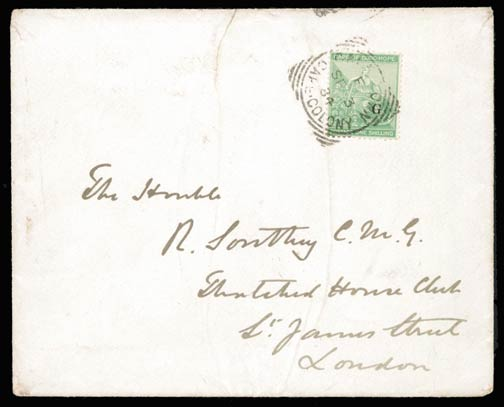
\includegraphics[width=.80\textwidth]{../tannu-tuva/cover-01.jpg}
\caption{RUSSIA TANNU TUVA }
\end{figure}




Some collectors contend that they did see at least some limited postal use.[6]
Notwithstanding their questionable origins, these exotic stamps were popular with young collectors during the middle of the twentieth century. This is documented, for example, in Ralph Leighton's Tuva or Bust!, Richard Feynman's Last Journey (W. W. Norton 1991), where childhood memories of the colorful stamps of Tannu Tuva inspired Nobel prize-winning physicist Richard Feynman and the author on a quest, first to contact someone in Tuva, and then to actually visit the country. (Feynman died before achieving his goal, but Leighton ultimately reached Tuva.)[9] Leighton and Feynman's efforts rekindled an interest in Tuva and its stamps, which now are the subject of numerous websites.

Since the 1990s, numerous labels purporting to be postage stamps of Tuva have again appeared on the market. These have depicted a variety of unlikely Tuvan subjects, such as Bart Simpson, the Teletubbies and Led Zeppelin, and are all illegal stamps apparently manufactured in England and intended to deceive collectors.[10]





http://www.tradewinds-co.com/ttpp/index.html



                                                    